\documentclass[11pt]{article}
\usepackage[margin=0.85in]{geometry}
\usepackage{graphicx}
\usepackage{booktabs}
\usepackage{xcolor}
\usepackage{hyperref}
\usepackage{float}
\usepackage{caption}
\captionsetup{font=small,skip=4pt}
\usepackage{titlesec}
\titlespacing*{\section}{0pt}{6pt}{2pt}
\titlespacing*{\subsection}{0pt}{4pt}{1pt}
\setlength{\parskip}{2pt}
\setlength{\parindent}{0pt}
\hypersetup{colorlinks=true, linkcolor=blue!50!black, urlcolor=blue!50!black}

\title{\vspace{-2.5em}Week 4: When LSP-Guided Rollback Helps (and When It Doesn't)\vspace{-0.6em}}
\author{\small CMSC 25750 quarter project}
\date{\vspace{-1.5em}\small 2026-04-20}

\begin{document}
\maketitle\vspace{-2.2em}

\paragraph{Setup.} We compare two arms on MultiPL-E HumanEval Rust across 15 open-weight models (0.8B--123B). \textbf{Arm A} = LSP + compiler: stream Rust, snapshot at each statement boundary, pull \texttt{rust-analyzer} native diagnostics, classify via the §6 procedure (position + class + open-fn demotion), abort on blocking errors and re-prompt. \textbf{Arm B} = compiler only: generate, \texttt{rustc}, retry on failure. Both bounded only by per-problem wall-clock (40--60\,s). Per-problem profiler logs 10 categories.

\paragraph{Hypotheses.} (H1) Arm A reaches first-pass-compile faster and with fewer compiler calls than Arm B. (H2) Partial scaling law: bigger models make fewer mistakes but take longer wall-clock. (H3) Coding-specialized models benefit less from rollback.

\begin{figure}[H]
\centering
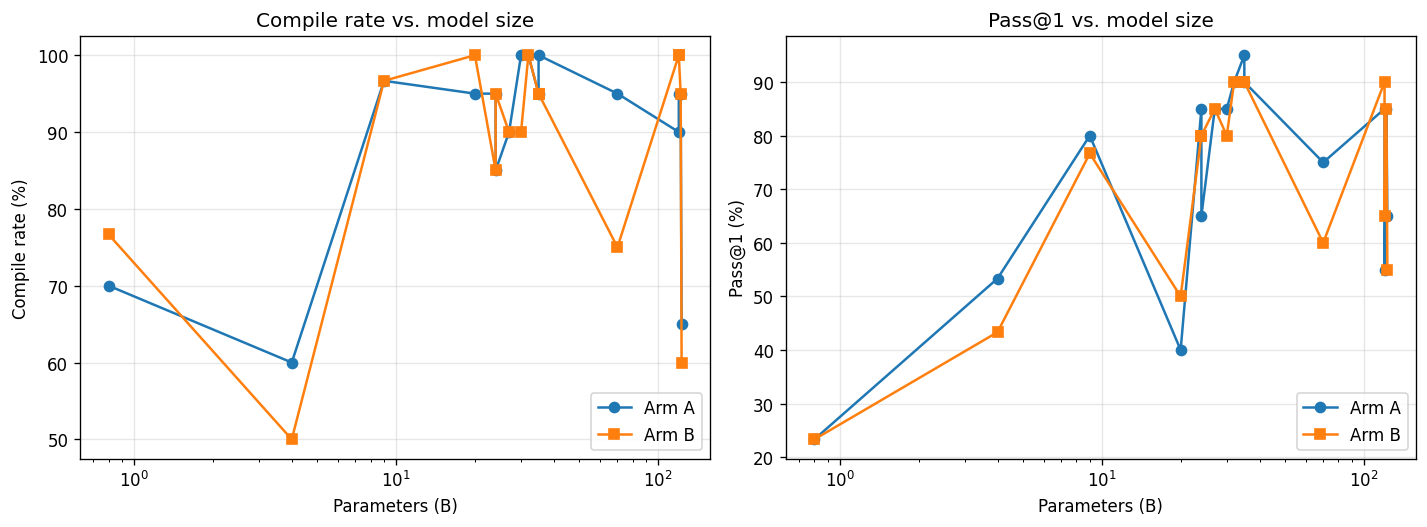
\includegraphics[width=0.49\linewidth]{../results/week4/plots/blog_pass_compile_by_size.png}\hfill
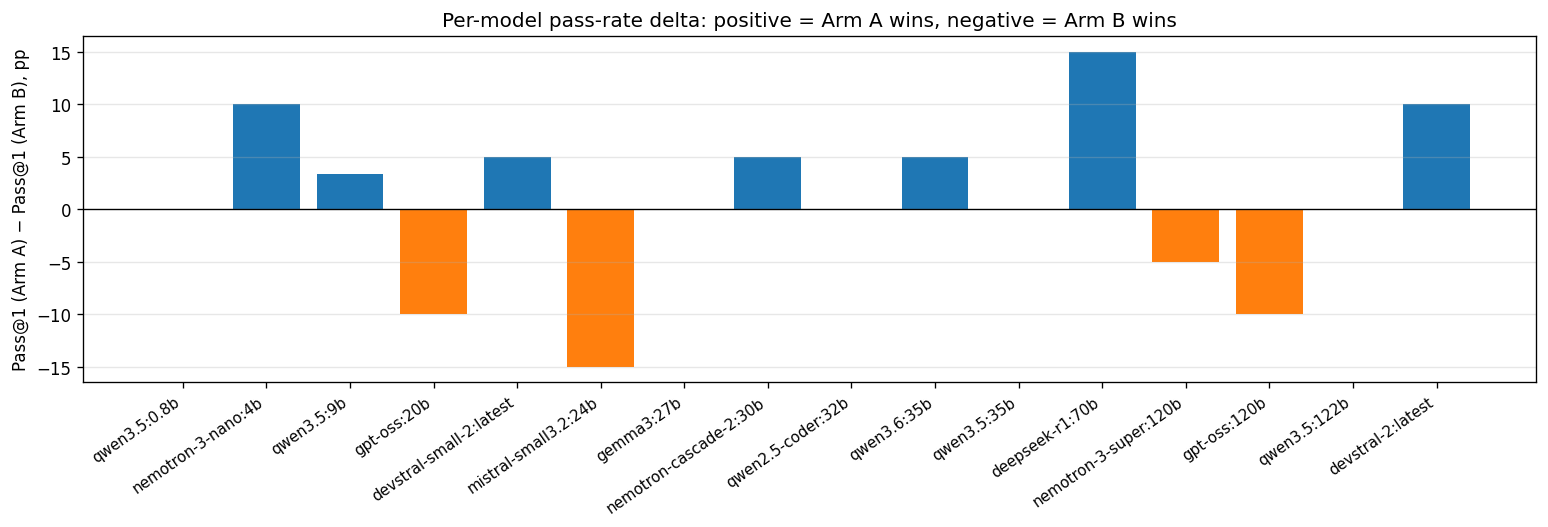
\includegraphics[width=0.49\linewidth]{../results/week4/plots/blog_arm_winners.png}
\caption{\textbf{Left:} compile/pass rates saturate by ${\sim}30$B; arm-wise gaps are loudest at the smallest models. \textbf{Right:} per-model pass-rate delta (Arm A $-$ Arm B), sorted by params. 5 models favor A clearly, 5 tied, 5 favor B — no monotone trend with size; stochastic variance in 20-problem samples dominates.}
\end{figure}

\paragraph{H1 falsified.} Wilcoxon signed-rank on paired wall-clock per problem: Arm A is significantly \emph{slower} than Arm B at \texttt{nemotron-3-nano:4b} ($p\!=\!0.0006$), \texttt{nemotron-cascade-2:30b} ($p\!=\!0.002$), \texttt{gpt-oss:20b} ($p\!=\!0.014$), \texttt{nemotron-3-super:120b} ($p\!=\!0.048$). No size shows A significantly faster. Median compiler calls per problem is \textbf{1.0 for both arms at every model} — A cannot reduce compiler calls because the LSP tier never blocks (see §Architectural).

\paragraph{H2 strongly supported on both arms.} Across 15 sizes (Spearman):
{\small
\begin{center}
\begin{tabular}{lcccc}
\toprule
& \multicolumn{2}{c}{\textbf{Arm A}} & \multicolumn{2}{c}{\textbf{Arm B}}\\
\cmidrule(lr){2-3}\cmidrule(lr){4-5}
& $\rho$ & $p$ & $\rho$ & $p$ \\
\midrule
params $\leftrightarrow$ compiler\_calls & $-0.61$ & $0.012$ & $-0.68$ & $0.004$ \\
params $\leftrightarrow$ wall-to-compile & $+0.51$ & $0.042$ & $+0.68$ & $0.004$ \\
\bottomrule
\end{tabular}\end{center}}

Both directions of the partial scaling law hold with $p<0.05$ on both arms.

\paragraph{H3 confirmed.} \texttt{qwen2.5-coder:32b}, \texttt{qwen3.5:35b}, \texttt{qwen3.6:35b} all $\geq$ 95\% compile / 90\% pass with $\leq$ 0.5 avg rollbacks. Arms statistically indistinguishable at this ceiling. Highest pass@1: \texttt{qwen3.6:35b} at \textbf{95\%}.

\paragraph{The architectural finding.} Across 15 models, 30 model-arm runs, 2,000+ classifier invocations, the LSP tier produced \textbf{zero} blocking classifications during real generation. Why? The §6 demotion rule downgrades \texttt{type-mismatch} (E0308) and \texttt{unresolved-reference} (E0425) to non-blocking when the fn body is open — necessary for forward-reference cases. But the body is always open during incremental generation, and these two codes dominate native diagnostic output on partial Rust. The classifier coverage and the demotion rule overlap almost exactly, leaving no signal to act on.

\paragraph{Positive control + confusion matrix.} To confirm the classifier is calibrated and not broken, I ran 24 hand-crafted snippets (8 closed real errors, 6 closed clean, 3 open with real error in completed stmt, 3 open with forward reference, 4 syntax-only):
{\small
\begin{center}
\begin{tabular}{lrrrrr}
\toprule
\textbf{Category} & \textbf{TP} & \textbf{FP} & \textbf{TN} & \textbf{FN} & \textbf{n} \\
\midrule
A — closed body, real semantic error & 8 & 0 & 0 & 0 & 8 \\
B — closed body, clean code & 0 & 0 & 6 & 0 & 6 \\
C — open body, real error in completed stmt & 2 & 0 & 0 & 1 & 3 \\
D — open body, forward reference & 0 & 0 & 3 & 0 & 3 \\
E — in-progress, syntax errors only & 0 & 0 & 4 & 0 & 4 \\
\midrule
\textbf{Total} & \textbf{10} & \textbf{0} & \textbf{13} & \textbf{1} & \textbf{24} \\
\bottomrule
\end{tabular}\end{center}}

\textbf{Precision = 1.00}, \textbf{specificity = 1.00}, \textbf{recall = 0.91}. The single FN is C1 (\texttt{type-mismatch} on a completed statement while fn body open) — the exact tradeoff §6 prescribes for avoiding forward-reference false alarms. The classifier is alive and correctly distinguishes the 5 categories. So the zero-blocking result during real generation is genuine: native diagnostics fire on Cat-C-style errors but the demotion suppresses them by design.

\paragraph{Conclusions and next step.} The null result on H1 is informative: external semantic verification with rollback runs into a tension between false-alarm avoidance (demote forward references) and fault detection (catch real type errors). MGD avoids it by using completions, not diagnostics. DSVD avoids it by using internal probes, not external LSP. Resolving the tension requires either selective demotion (don't demote \texttt{type-mismatch}, only \texttt{unresolved-reference}) or replacing native diagnostics with incremental \texttt{cargo check} — slower per call but ground-truth, no demotion needed. Week 5 will migrate to HuggingFace \texttt{transformers} (eliminating the 3--5\% Ollama rollback-overhead) and test these redesigns.

\textbf{Code}: \texttt{soundcode/eval/} (15 modules, 99 tests passing). \textbf{Data}: 30 result JSONs + 700 per-problem profiles in \texttt{results/week4/}. \textbf{Validation}: \texttt{classifier\_positive\_control.py}, \texttt{classifier\_confusion.py}.

\end{document}
